%%
%
% ARQUIVO: cap-01.tex
%
% VERSÃO: 1.0
% DATA: Maio de 2016
% AUTOR: Coordenação de Trabalhos Especiais SE/8
% 
%  Arquivo tex de exemplo de capítulo do documento de Projeto de Fim de Curso.
%
% ---
% DETALHES
%  a. todo capítulo deve começar com \chapter{•}
%  b. usar comando \noindent logo após \chapter{•}
%  c. citações para referências podem ser
%       i. \citet{•} para citações diretas (p. ex. 'Segundo Autor (2015)...'
%       ii. \citep{•} para citações indiretas (p. ex. '... (AUTOR, 2015)...'
%  d. notas de rodapé devem usar dois comandos
%       i. \footnotemark para indicar a marca da nota no texto
%       ii. \footnotetext{•}, na sequência, para indicar o texto da nota de rodapé
%  e. figuras devem seguir o exemplo
%       i. devem ficar no diretório /img e devem ser no formato EPS
%  f. tabelas devem seguir o exemplo
%  g. figuras e tabelas podem ser colocadas em orientação landscape
%       i. figuras: usar \begin{sidewaysfigure} ... \end{sidewaysfigure}
%                   em vez de \begin{figure} ... \end{figure}
%       ii. tabelas: usar \begin{sidewaystable} ... \end{sidewaystable}
%                    em vez de \begin{table} ... \end{table}
%  h. toda figura e tabela deve ser referenciada ao longo do texto com \ref{•}
% ---
%%

\chapter{Introdução}

\section{Motivação}
Cada vez mais as máquinas estão sendo utilizadas em atividades de nossa sociedade. Atuando na substituição de profissionais ou no auxílio dos mesmos, elas estão presentes e participando de nosso cotidiano ativamente. A implementação de sistemas de visão computacional tem se tornado, portanto, uma necessidade mais forte à medida que as aplicações que envolvem o tratamento de imagens se desenvolvem e buscam se aproximar da visão e da análise humana.
A segmentação é uma importante técnica utilizada nas atividades que envolvem o processamento digital de imagens. Diversas são as aplicações que fazem uso da identificação e análise de uma imagem, necessitando do estudo de regiões específicas das mesmas a fim de alcançar resultados e conclusões de forma eficiente.
Por se tratar de um problema sem solução universal e de vasta aplicação,  existem inúmeras possibilidades a serem exploradas e muito se tem estudado sobre essa área, com a evolução de novas técnicas e algoritmos que trazem uma nova abordagem ao problema.
%Esse projeto trará, portanto, um conhecimento mais profundo nesse importante domínio da Visão Computacional com a concepção de um produto que servirá tanto como base para estudo quanto uma base para futuros projetos mais avançados.
Esse projeto visa estudar e implementar técnicas de segmentação de imagens no ambiente Android, possibilitando o aprendizado de diferentes métodos da área de processamento de imagens, incluindo a área de visão computacional, bem como de desenvolvimento de aplicativos na plataforma Android. A Figura \ref{fig:tela_android} exibe o resultado do aplicativo que este projeto de final de curso está desenvolvendo.


% Figura -----------------------------------------------------------------------------------------------------------------------------
  \begin{figure}[!htb]
       \begin{center}  
          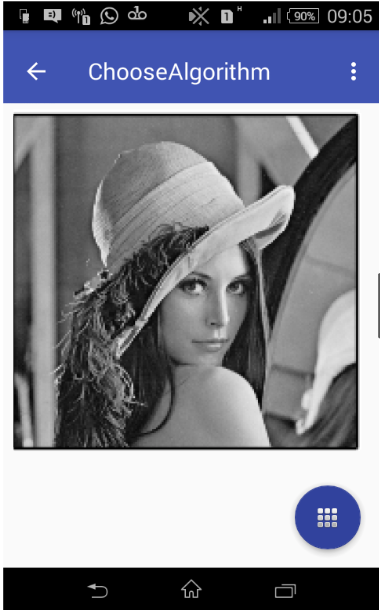
\includegraphics[width=0.2\columnwidth]{img/tela_android-original.png} \quad
          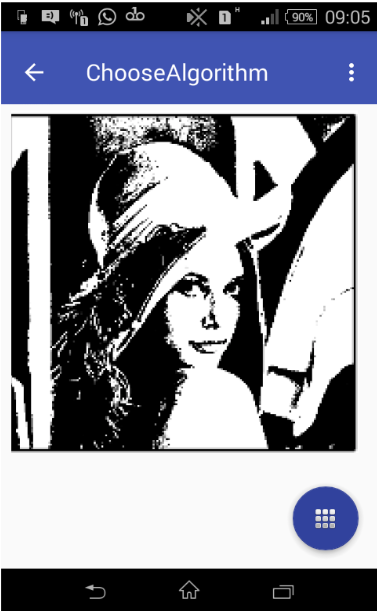
\includegraphics[width=0.2\columnwidth]{img/tela_android.png}
           \caption{\label{fig:tela_android}Tela do Aplicativo Android (imagem original e imagem segmentada).}
           % \vspace{2.0em}
       \end{center}
   \end{figure}
 % Figura -----------------------------------------------------------------------------------------------------------------------------

% um conhecimento mais profundo nesse importante domínio da Visão Computacional com a concepção de um produto que servirá tanto como base para estudo quanto uma base para futuros projetos mais avançados.


\section{Objetivos}
O objetivo dessa pesquisa é o desenvolvimento de uma aplicação móvel, em plataforma Android, capaz de segmentar imagens por meio de diferentes algoritmos e técnicas de pré-processamento na área de Visão Computacional. A realização de todas as etapas de desenvolvimento até a concepção do produto final, que será disponibilizado para livre utilização, permitirá aos alunos maior conhecimento nesse assunto que é um dos domínios mais promissores da tecnologia e complementará a sua formação como engenheiros de Computação. A Figura \ref{fig:diag_blocos} ilustra os passos do projeto, onde o aplicativo poderá adquirir imagens diretamente da câmera do dispositivo ou da galeria de imagens do dispositivo. O bloco denominado Pré-Processamento ilustra uma possível etapa de pré-processamento das imagens oriundas da câmera ou do banco de imagens, com a finalidade de tratar as imagens para os algoritmos de segmentação. O bloco seguinte, Técnicas de Segmentação implementa um ou mais métodos de segmentação, descritos no capítulo \ref{cap:segmentacao}. Finalmente, o bloco Exibição vai exibir a imagem segmentada na tela do dispositivo. 

% Figura -----------------------------------------------------------------------------------------------------------------------------
  \begin{figure}[!htb]
       \begin{center}  
          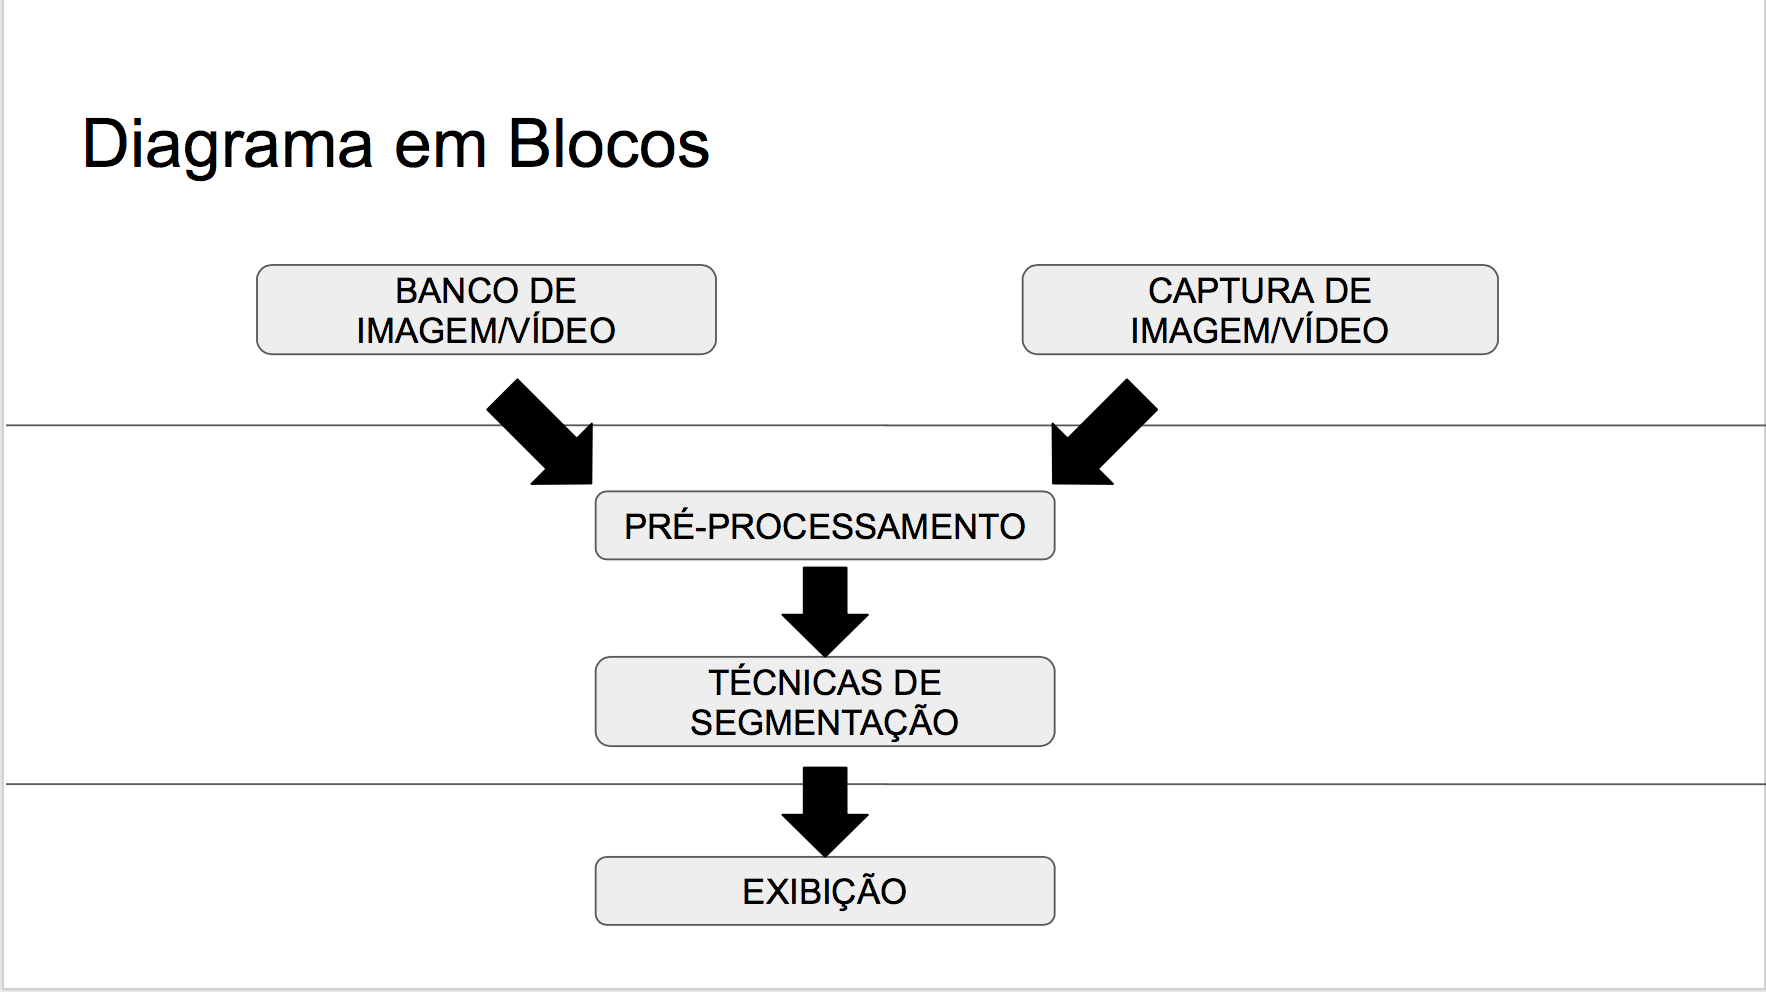
\includegraphics[width=0.7\columnwidth]{img/diag_blocos.png}
           \caption{\label{fig:diag_blocos}Diagrama em Blocos do Projeto.}
           % \vspace{2.0em}
       \end{center}
   \end{figure}
 % Figura -----------------------------------------------------------------------------------------------------------------------------


\section{Justificativa}
Este trabalho pode ser justificado com base nos seguintes pontos:
\begin{itemize}
\item Inexistência de uma solução única para o problema em questão. Trata-se de um problema ainda em aberto com muitas oportunidades a serem exploradas;
\item Diversas aplicações necessitam da segmentação de imagens como parte importante das suas atividades, além de outras que podem ser aprimoradas e desenvolvidas por meio de sua utilização;
\item Visão computacional como domínio promissor da tecnologia, com uma atuação cada vez maior no mercado e interação com outros domínios como robótica e inteligência artificial.
\end{itemize}

\chapter{Segmentação de Imagens}\label{cap:segmentacao}
A segmentação é um problema do tipo "ill-posed" ("mal definido"), uma vez que não existe uma solução única, universal. Por isso, a segmentação é considerada o problema mais difícil de ser resolvido em análise de imagens \citep{Poggio1985}.

\section{Conceito}
A segmentação de imagens tem como uma de suas interpretações como a divisão em regiões ou categorias consideradas "relevantes", que correspondem a objetos ou partes de objetos. Decidir o que é relevante em uma imagem depende do problema a ser resolvido, em que os objetos segmentados devem corresponder às áreas de interesse da aplicação. Dentre essas aplicações, podemos citar os seguintes exemplos:

\begin{itemize}
\item Aplicações militares: Reconhecimento de alvos terrestres, aéreos e navais;
\item Análise de imagens médicas: Identificação de doenças como tumores;
\item Veículos autônomos;
\item Robótica.
\end{itemize}

\section{Segmentação para seres humanos e para computadores}
Para seres humanos, a identificação de regiões similares ou objetos diferentes presentes em uma imagem é um processo fácil. Nosso sistema cognitivo auxiliado por nosso sistema visual nos permite reconhecer e segmentar os objetos de forma instantânea sem nos darmos conta desse processo. Além disso, usamos a segmentação por distância como técnica auxiliar , uma vez que nossa visão estereoscópica nos fornece informação de profundidade.
No caso de computadores, essa tarefa se torna mais complexa, pois envolve a análise de características de cada pixel ou da distribuição da população de pixels. Para isso, deve-se implementar algoritmos de segmentação, os quais serão explorados com maior profundidade nas seções subsequentes dessa pesquisa. A Figura \ref{fig:Berkeley_mulher} exibe uma imagem que foi manualmente segmentada por 4 seres humanos. É possível notar que cada pessoa não identificou como "relevantes" as mesmas áreas, conforme ilustrado pela Figura \ref{fig:Berkeley_mulher_segmentada}. 

% Figura 
  \begin{figure}[!htb]
       \begin{center}  
          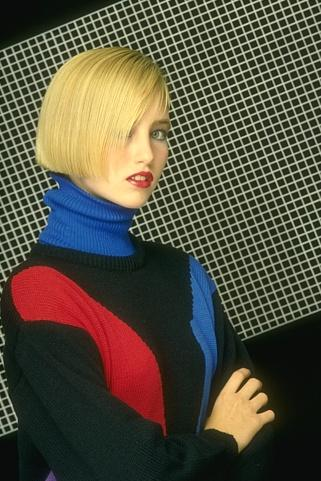
\includegraphics[width=0.3\columnwidth]{img/198023.jpg}
           \caption{\label{fig:Berkeley_mulher}Imagem original\citep{Arbelez2011}.}
           % \vspace{2.0em}
       \end{center}
   \end{figure}

 % Figura 
\begin{figure}[!htb]
 \centering
 \def\baselinestretch{1}\small\normalsize
 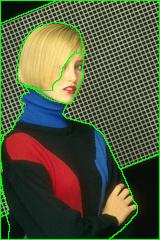
\includegraphics[width=0.2\textwidth]{img/198023-8-color.jpg}\qquad
 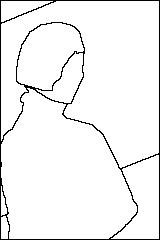
\includegraphics[width=0.2\textwidth]{img/198023-8.jpg}  \qquad
  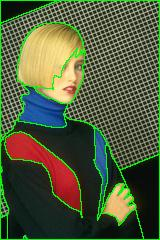
\includegraphics[width=0.2\textwidth]{img/198023-16-color.jpg}  \qquad
 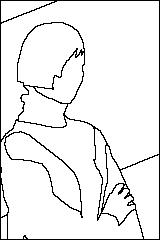
\includegraphics[width=0.2\textwidth]{img/198023-16.jpg}        
 \caption{\label{fig:Berkeley_mulher_segmentada}Imagens segmentadas por seres humanos, gerando 8 e 16 segmentos nas duas primeiras imagens e nas duas últimas, respectivamente.\citep{Arbelez2011}.}
 %\vspace{2.0em}
\end{figure}


% Figura 
\begin{figure}[!h]
 \centering
 \def\baselinestretch{1}\small\normalsize
 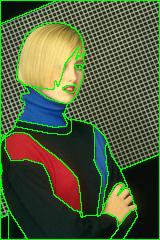
\includegraphics[width=0.2\textwidth]{img/198023-22-color.jpg}\qquad
 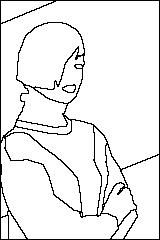
\includegraphics[width=0.2\textwidth]{img/198023-22.jpg}  \qquad
  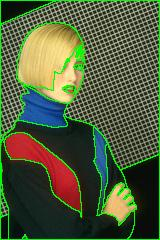
\includegraphics[width=0.2\textwidth]{img/198023-26-color.jpg}  \qquad
 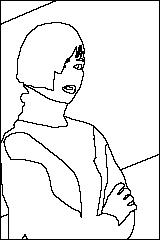
\includegraphics[width=0.2\textwidth]{img/198023-26.jpg}        
 \caption{\label{fig:Berkeley_mulher_segmentada}Imagens segmentadas por seres humanos, gerando 22 e 26 segmentos nas duas primeiras imagens e nas duas últimas, respectivamente.\citep{Arbelez2011}.}
 %\vspace{2.0em}
\end{figure}




Ainda que o processo de segmentação para humanos seja fácil e automático, é comum e natural que diferentes pessoas identifiquem objetos ou partes de objetos distintos em uma dada imagem. Isso se deve à percepção de relevância atribuída a cada região variar com a interpretação pessoal de cada um. 
O mesmo problema ocorre de forma mais acentuada com relação aos diferentes algoritmos. Cada algoritmo tem a sua própria abordagem para tratar do mesmo problema e, de acordo com sua implementação, leva a diferentes resultados, que podem ser analisados comparativamente. É importante dizer que o mesmo algoritmo pode ser mais ou menos eficiente de acordo com a imagem utilizada como dado de entrada, possibilitando diversos estudos na área como o tema desta pesquisa. A Figura \ref{fig:indio} ilustra este problema\citep{berkeley} . 

% Figura 
  \begin{figure}[!htb]
       \begin{center}  
          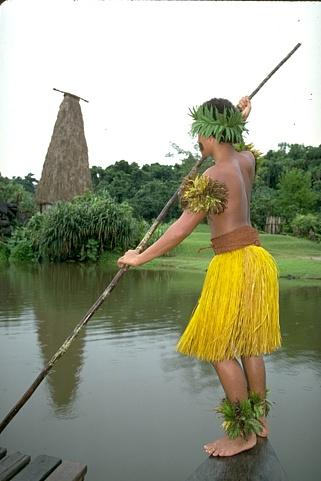
\includegraphics[width=0.3\columnwidth]{img/101087.jpg}
           \caption{\label{fig:Berkeley_mulher}Imagem original\citep{berkeley}.}
           % \vspace{2.0em}
       \end{center}
   \end{figure}



 % Figura -----------------------------------------------------------------------------------------------------------------------------       
\begin{figure}[!htb]
 \centering
 \def\baselinestretch{1}\small\normalsize
 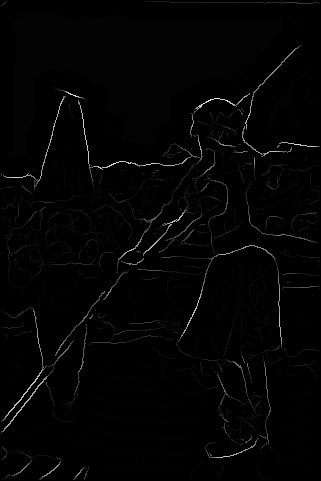
\includegraphics[width=0.2\textwidth]{img/101087-77.jpg}\qquad
 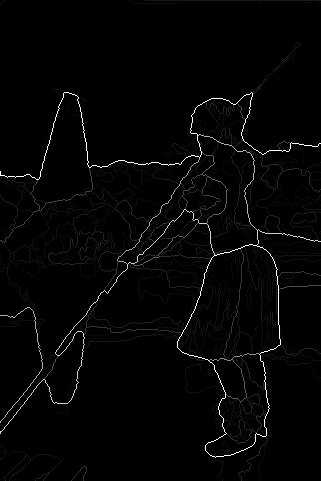
\includegraphics[width=0.2\textwidth]{img/101087-80.jpg}  \qquad 
  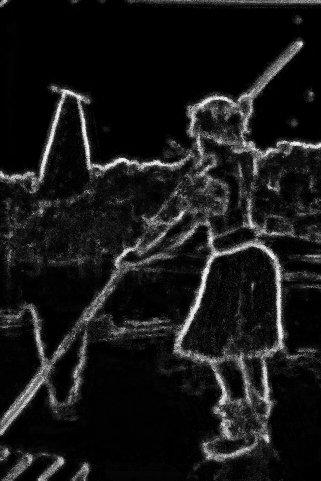
\includegraphics[width=0.2\textwidth]{img/101087-82.jpg}  \qquad
 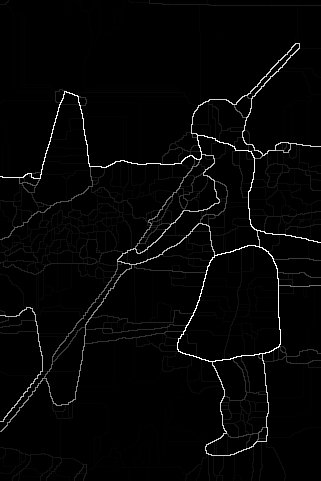
\includegraphics[width=0.2\textwidth]{img/101087-85.jpg}        
 \caption{\label{fig:indio}Resultados de 4 algoritmo de detec\c{c}\~{a}o de bordas \citep{berkeley}.}
 %\vspace{2.0em}
\end{figure}
 % Figura -----------------------------------------------------------------------------------------------------------------------------



Devido a  grande variedade de algoritmos existentes, nos limitaremos à explicação dos principais e mais utilizados, os quais fornecem um bom entendimento das técnicas utilizadas e servem como base para o desenvolvimento de novas técnicas. O Capitulo \ref{cap:algoritmos} apresenta as técnicas estudadas.



\chapter{Algoritmos de Segmentação}\label{cap:algoritmos}

Este capitulo descreve 4 técnicas de segmentação de imagens, sendo a por limiar (Thresholding) a mais simples. As técnicas baseadas em bordas e regiões são mais complexas e demandam um ônus computacional mais elevado.

% \section{Tipos de Algoritmos}
\begin{itemize}
    \item Thresholding
    \item Método Baseado em Bordas 
    \item Método Baseado em Regiões
    \begin{itemize}  
        \item Split and Merge
        \item Watershed
    \end{itemize}
\end{itemize}

\subsection{Thresholding}
É o método mais simples de segmentação de imagens.
Busca dividir a imagem em duas categorias: objetos (foreground) e background. 
Cada pixel é alocado a uma categoria de acordo com seu valor em níveis de cinza.

Dado um threshold T, o pixel localizado na posição (i,j) com valor fij é alocado à categoria 1 se: fij $\leq$ T.Caso contrário, o pixel é alocado à categoria 2.

O threshold T pode ser escolhido manualmente, tentando diferentes valores de T e analisando qual deles é mais eficiente na identificação dos objetos de interesse.
O threshold T também pode ser escolhido a partir do Histograma da imagem.

Escolhe-se T como o valor entre as duas distribuições de cinza.

\textcolor{red}{EXEMPLOS}

\subsection*{Threshold Global}
O mesmo valor de T é usado para a imagem inteira.

\subsection*{Threshold Local (ou dinâmico)}
Divide-se a imagem em regiões distintas e adota-se um valor T para cada uma delas, onde esse valor funcionará como Threshold Global.

\subsection{Baseado em Bordas}
Primeiramente, classifica-se os pixels como “borda” ou “não-borda”.
Depois, divide-se a imagem em regiões, baseado nas bordas detectadas.

As bordas são identificadas por meio das descontinuidades, isto é, variações abruptas nos valores dos pixels. 

\textcolor{red}{EXEMPLOS e as REFERENCIAS, se for o caso}


\subsection{Baseado em Regiões}
\subsubsection*{O que é uma região?}
Uma região pode ser “definida” como um grupo de pixels conectados com propriedades similares.
Porém, é um conceito importante e difícil de definir, já que depende da interpretação do que seria uma região  em determinado caso, conforme ilustrado no capitulo \ref{cap:segmentacao} pelas Figuras \ref{fig:Berkeley_mulher_segmentada} e \ref{fig:indio}.

\textcolor{red}{EXEMPLOS}

\subsubsection{Split and Merge}
\subsubsection*{Procedimento}
As etapas fundamentais deste algoritmo segundo  são: 
\begin{enumerate}
    \item Criar critério para definir o que é uma área homogênea.
    \item Começar com a imagem completa e divide em 4 sub-imagens.
    \item Checar cada sub-imagem e dividi-la novamente em 4 novas sub-imagens caso ela não seja homogênea.
    \item Repetir Passo 3 até que não se consiga mais subdividir.
    \item Comparar sub-imagens com suas regiões vizinhas e agrupá-las se forem homogêneas.
    \item Repetir Passo 5 até que não se consiga mais agrupar.
\end{enumerate}
Um exemplo de segmentação baseada em região Split and Merge é o algoritmo quadtree.


\subsubsection{Region growing (abordagem bottom-up)}
\subsubsection*{Procedimento}
As etapas fundamentais deste algoritmo são: 
\begin{enumerate}
    \item Identificar o ponto de partida.
    \item Incluir pixels vizinhos com características similares (nível de cinza, textura, cor, etc).
    \item Continuar até que todos os pixels estejam associados com um dos pontos de partida.
\end{enumerate}

\subsubsection*{EXEMPLO - WATERSHEED}
Um exemplo de segmentação baseada em região Region growing é o algoritmo watershed. A figura \ref{fig:coins} abaixo ilustra a segmentação de imagem por este algoritmo, e observa-se que regiões distintas correspondentes à cada moeda da figura.

% ------------------------------------------------------------------------------------------------------------
% Figura 
\begin{figure}[!htb]
 \centering
 \def\baselinestretch{1}\small\normalsize
 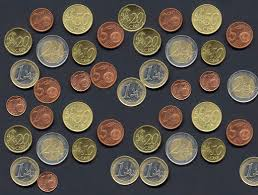
\includegraphics[width=0.4\textwidth]{img/stf-coins.jpg}\qquad
 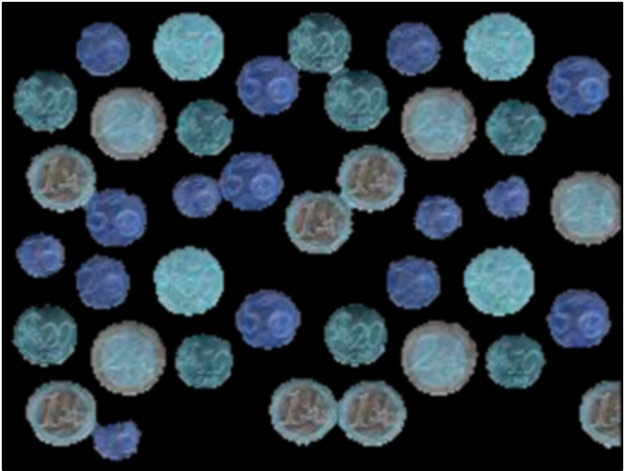
\includegraphics[width=0.4\textwidth]{img/stf-coins-watersheed.jpg} 
 \caption{\label{fig:coins}Imagem de uma moeda \citep{stanford} à esquerda e à direita segmentada pelo algoritmo watersheed em linguagem de programação python.}
 %\vspace{2.0em}
\end{figure}
 
% Stanford DataSet
%  https://scien.stanford.edu/index.php/test-images-and-videos/
 


\chapter{Ferramentas}

\textcolor{red}{OpenCV e Android}


\chapter{Cronograma}
\section{Definição de Etapas}
\subsection{Escolha do Tema e Estudo de Viabilidade}
A escolha do tema foi a primeira etapa do projeto. O uso de dispositivos móveis, bem como de suas respectivas câmeras tem sido cada dia mais frequentes. Essas câmeras captam informações do ambiente que os cercam e a segmentação de imagem pode ser usado no processamento de imagens de forma a desenvolver soluções computacionalmente automatizáveis.

Após a escolha do tema, foi feito o estudo de viabilidade, de forma a se verificar a possibilidade da cumprimento do objetivo do tema em tempo aceitável.

\subsection{Revisão Bibliográfica}
Rêferencias tais como livros, artigos e outras referências foram estudadas durante o período de revisão bibliográfica, de forma a permitir um embasamento bibliográfico do projeto.

\subsection{Elaboração da Monografia}
Esta fase do projeto se estende até o termino do projeto de fim de curso. Nesta última, confecciona-se um relatório utilizando-se os conhecimentos adquiridos desde o início do projeto.

\subsection{Estudo e Análise dos Algoritmos de Segmentação de Imagem}
Na aplicação proposta, alguns algoritmos de segmentação de imagem serão implementados no dispositivo móvel, de modo a estudá-los e verificar o mais apropriado à aplicação.

\subsection{Implementação}
A implementação ocorrerá após o estudo dos algoritmos e da definição de quais deles são mais indicados à proposta. Em uma primeira fase os algoritmos serão implementados em outros ambientes de desenvolvimento e em uma segunda etapa será realizada a portabilidade para o ambiente Android.

\subsection{Teste}
Os testes com as imagens em diferentes algoritmos serão realizados e, com a implementação pronta, pode-se observar e comparar os resultados dos algoritmos.

\subsection{Entrega do Relatório Final e Apresentação}
A partir das análises e de todo conteúdo, implementação, análises e testes, será feito o relatório e a apresentação à banca.


\section{Entregáveis}
Os entregáveis serão:

\begin{itemize}
\item Projeto do  Aplicativo
\item Escolha dos Algoritmos 
\item Aplicativo em Ambiente Android de Segmentação de Imagens implementado
\item Testes e análises comparativas
\end{itemize}

%Os dois primeiros ítens serão entregues durante a apresentação da Verficação Corrente (VC),e os outros serão entregues por ocasião da apresentação da Verificação Final (VF).

\begin{table}[!htpb]
\centering

% definindo o tamanho da fonte para small
% outros possíveis tamanhos: footnotesize, scriptsize
\begin{small} 
  
% redefinindo o espaçamento das colunas
\setlength{\tabcolsep}{3pt} 

% \cline é semelhante ao \hline, porém é possível indicar as colunas que terão essa a linha horizontal
% \multicolumn{10}{c|}{Meses} indica que dez colunas serão mescladas e a palavra Meses estará centralizada dentro delas.

\begin{tabular}{|c|c|c|c|c|c|c|c|c|c|c|}\hline
 & \multicolumn{9}{c|}{Meses}\\ \cline{2-10}
\raisebox{1.5ex}{Etapa} & FEV & MAR & ABR & MAI & JUN & JUL & AGO & SET & OUT \\ \hline

4.1.1 & X & X & X & & & & & &   \\ \hline
4.1.2 & X & X & X & X & & & & &   \\ \hline
4.1.3 & X & X & X & X & X & X & X & X & X    \\ \hline
4.1.4 & &  &  & &  & X & X & X &  \\ \hline
4.1.5 & &  &  & &  & X & X & X &    \\ \hline
4.1.6 & & & & & & & & X &   \\ \hline
4.1.7 & & & & & & & & & X  \\ \hline

\end{tabular} 
\end{small}
\caption{Cronograma das atividades previstas}
\label{t_cronograma}
\end{table} 

%\chapter{REFRÊNCIAS BIBLIOGRÁFICAS}
%\begin{itemize}
%    \item GLOCKSTEIN, Bob. Quadtrees and Octrees. Disponível em: <http://euklid.mi.uni-koeln.de/c/mirror/www.cs.curtin.edu.au/units/cg351-551/notes/lect51.html>. Acesso em: 10 mai. 2017
%    \item Chris. Segmentation. Disponível em: <http://www.bioss.ac.uk/people/chris/ch4.pdf>. Acesso em: 10 mai. 2017
%    \item STRAND, Robin. Segmentation. Disponível em: <http://www.it.uu.se/edu/course/homepage/\\bild1/ht14/L6\_segmentation.pdf>. Acesso em: 10 mai. 2017
%\end{itemize}





